%!TEX root = ../../terrainbook.tex
% chktex-file 46

\graphicspath{{appendices/normalplane/figs/}}

\chapter{Estimating the normals in a point cloud}%
\label{app:normalplane}

\begin{marginfigure}
  \centering
  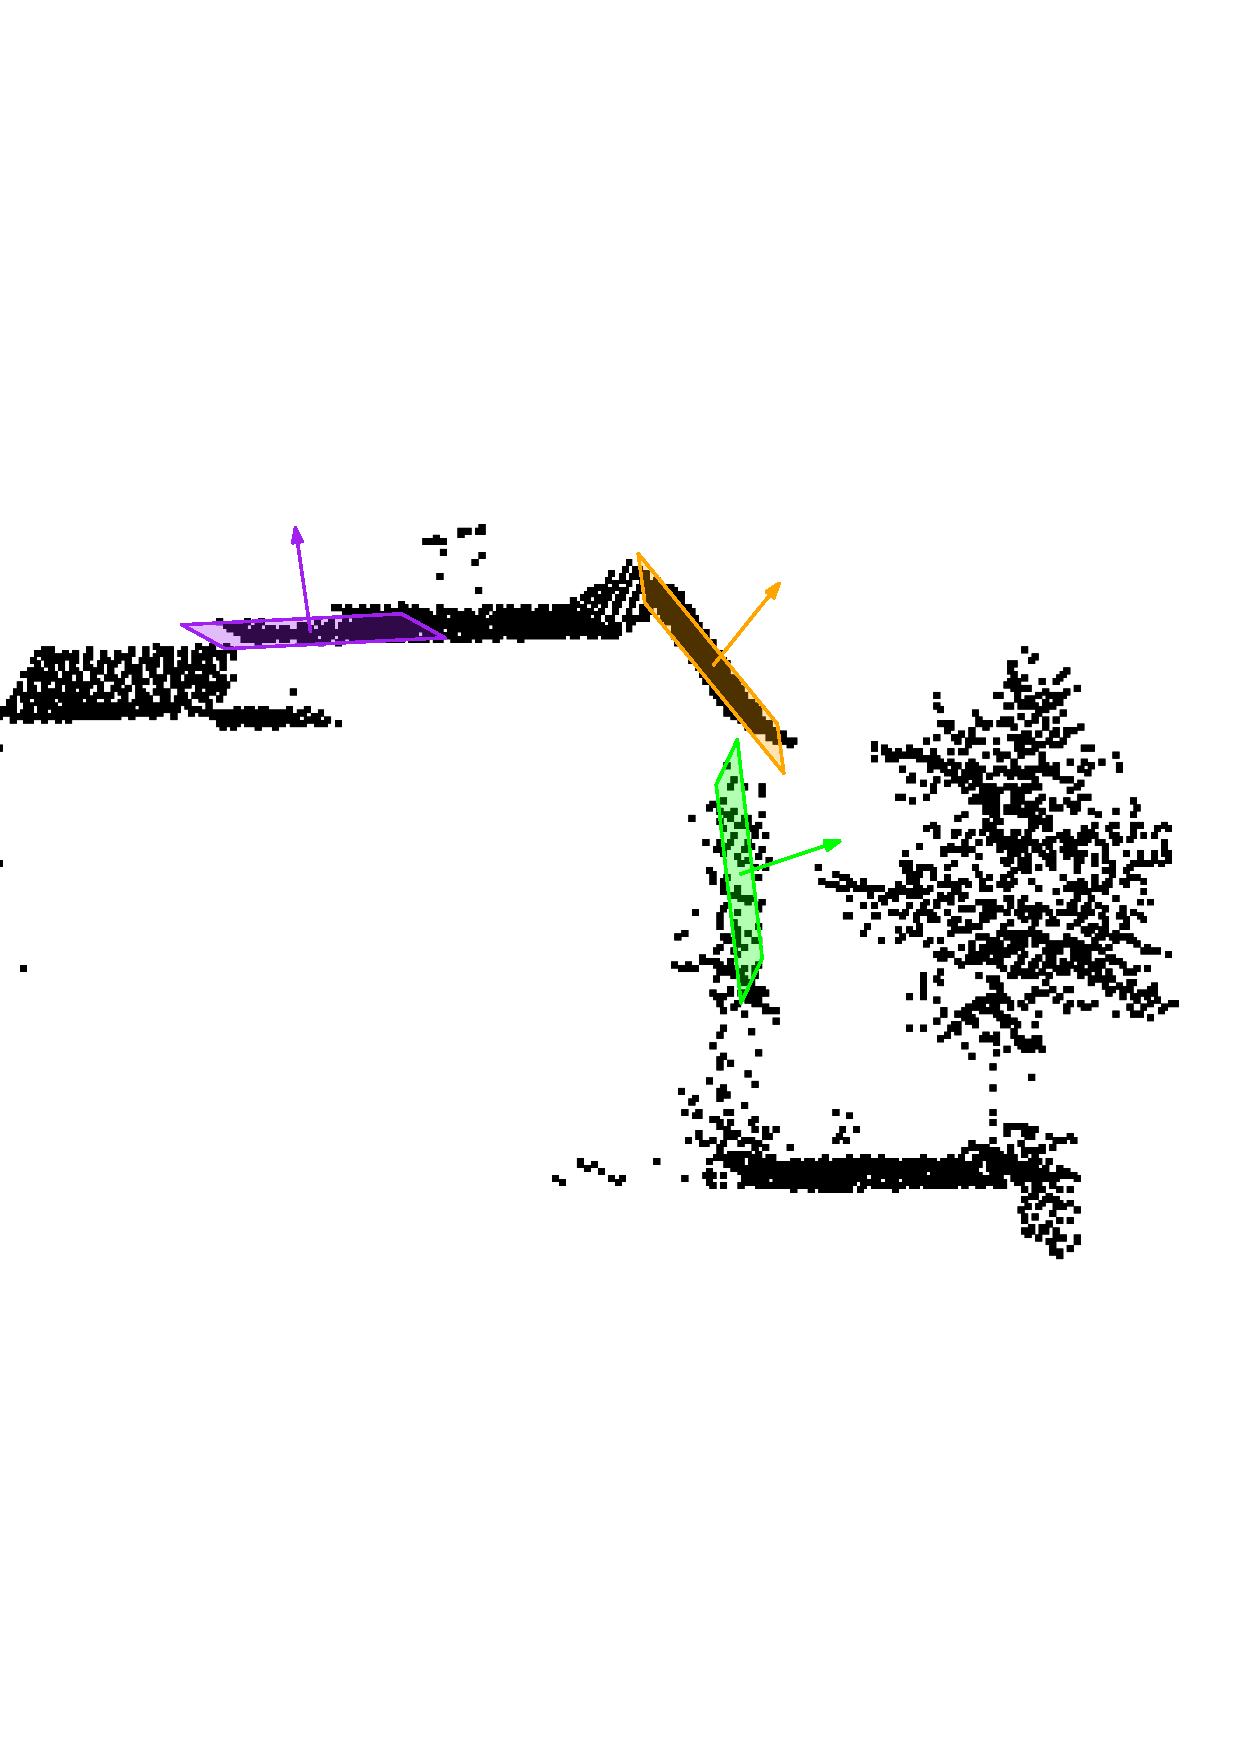
\includegraphics[width=\linewidth]{normal_demo.pdf}
  \caption{Perspective view of a point cloud with 3 plane fitted and their normal vector.}%
\label{fig:normal_demo}
\end{marginfigure}

Given a point cloud $S$, the normal vector for a point $p \in S$ can be found by fitting a plane $P$ to the points in the local neighbourhood of $p$. 
The vector orthogonal to this plane is the normal vector $\vec{n}$ of $p$.

In practice, we might want to use the 10 (or 15 or 20, depending on the resolution of $S$) nearest neighbours to $p$.
This can be efficiently (and easily with the many implementations available) performed with a $k$d-tree, see Section~\ref{sec:knn-m}.

To fit the plane, the preferred option is to use least-square fitting because it minimises the sum of squared distances between the points and the plane $P$.

We suggest to use Principal Component Analysis (PCA) 
\marginnote{Principal Component Analysis (PCA)}%
\index{Principal Component Analysis (PCA)}
to obtain the plane $P$, and to obtain its normal $\vec{n}$.
PCA allows us to identify the directions of maximum variance in a dataset, and it uses the \emph{eigenvalues} and \emph{eigenvectors} of the covariance matrix of a dataset.
\marginnote{eigenvalues and eigenvectors}%
\index{eigenvalues}\index{eigenvectors}
The eigenvector linked with the largest eigenvalue represents the direction where the variance is the largest, and the smallest eigenvalue where the variance is the smallest.

%

For our subset of 10 or 15 neighbouring points in $S$, the direction of maximum variance is the plane that best fits the data, and the normal vector is the direction of minimum variance.
Figure~\ref{fig:knn_normal} shows that one should be careful for points close to the edges of building for instance, since the normal will be affected by neighbouring points.
\begin{marginfigure}
  \centering
  \begin{subfigure}[b]{\linewidth}
    \centering
    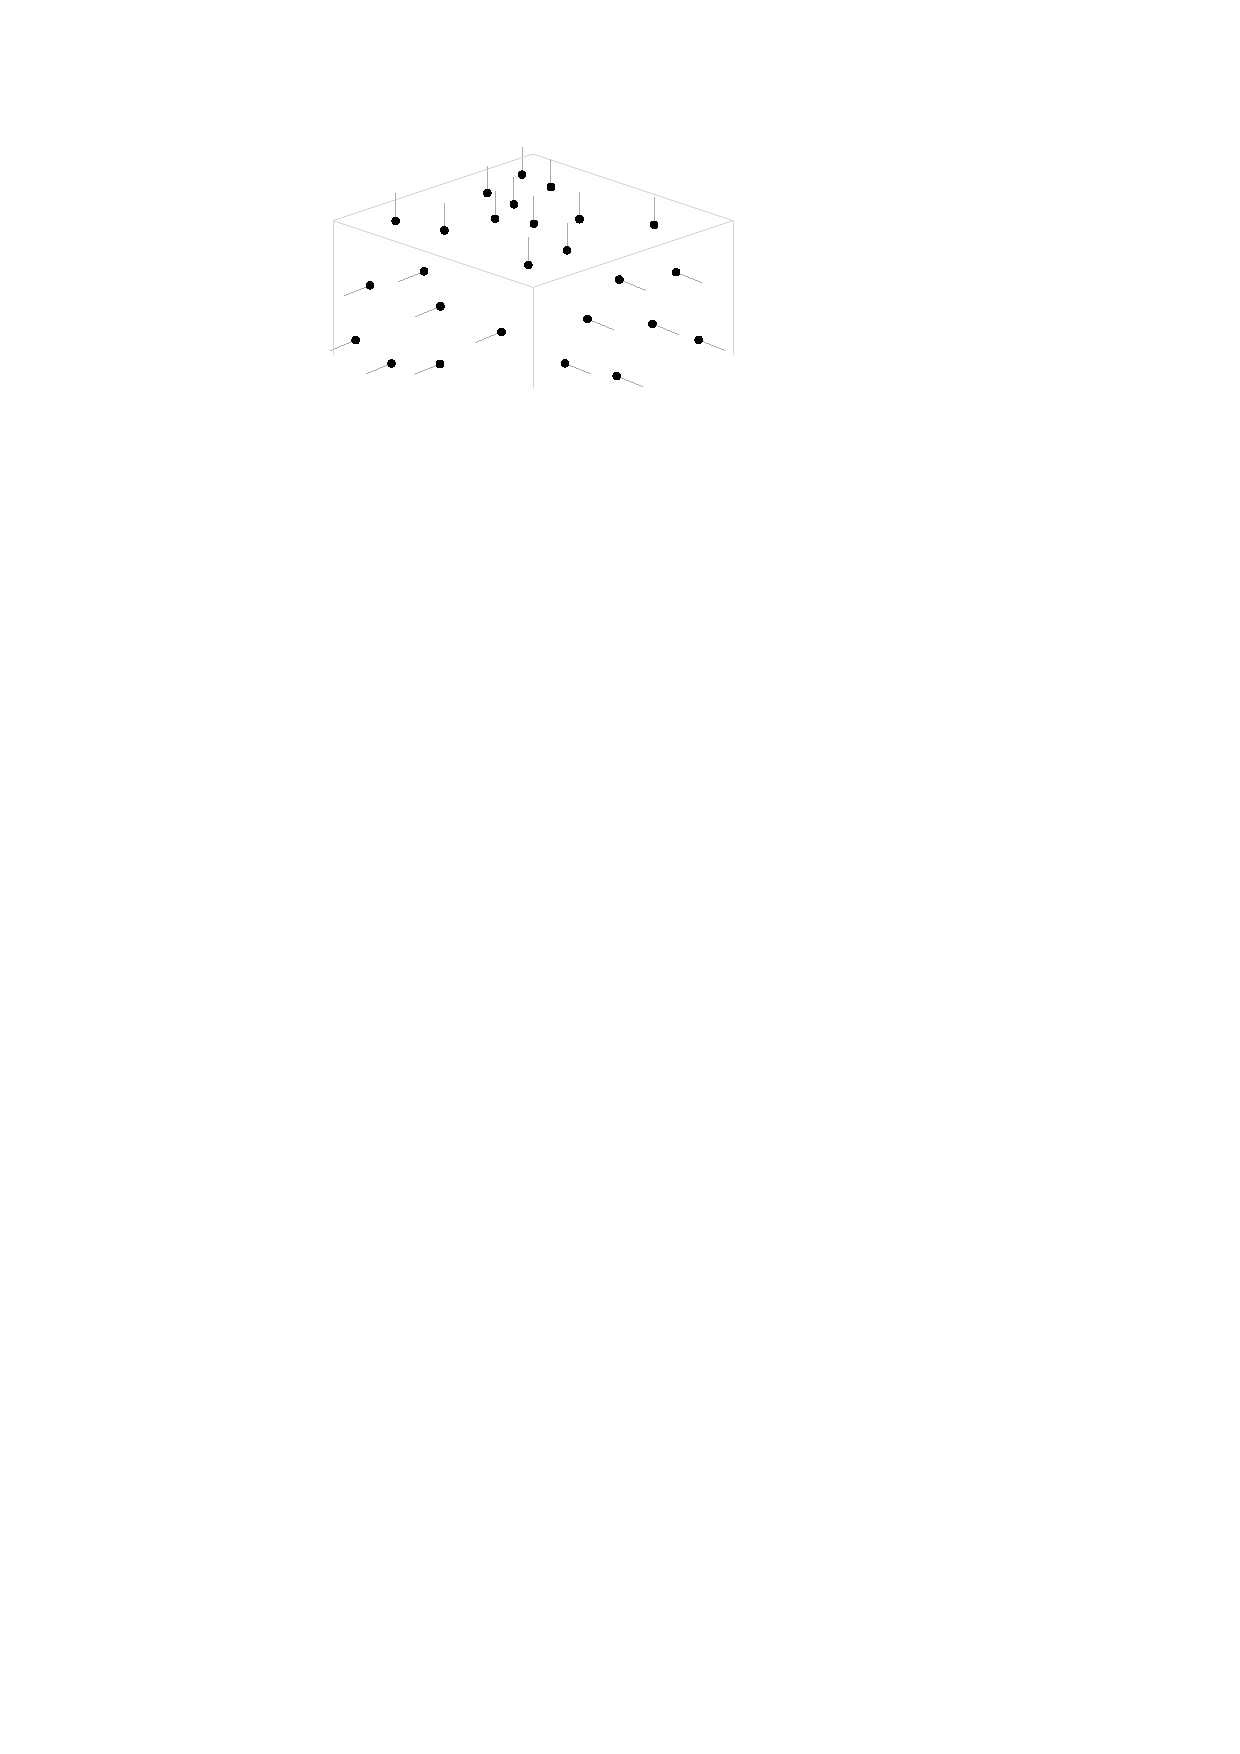
\includegraphics[width=\textwidth,page=1]{normal.pdf}
    \caption{}\label{fig:normal:a}
  \end{subfigure}
  \qquad
  \begin{subfigure}[b]{\linewidth}
    \centering
    \includegraphics[width=\textwidth,page=2]{normal.pdf}
    \caption{}\label{fig:normal:b}
  \end{subfigure}
  \qquad
  \begin{subfigure}[b]{\linewidth}
    \centering
    \includegraphics[width=\textwidth,page=3]{normal.pdf}
    \caption{}\label{fig:normal:c}
  \end{subfigure}
  \caption{Calculating the normal of points with $k$d-trees and fitting of a plane. \textbf{(a)} A few points sampling the surface of a cube. \textbf{(b)} For the case where 5 neighbours are used, the normal is indicated in dark red. \textbf{(c)} If $p$ is near the edge of the cube, then some neighbours will on the other face and the normal will be modified.}%
\label{fig:knn_normal}
\end{marginfigure}

%

Observe that the normal obtain this way is not by definition correctly oriented, that is it could point in either direction perpendicular to the fitted plane.
For buildings, we usually prefer to have the normal pointing outwards/up, and thus the normal with the $z$-component positive is usually chosen.

%%%
%
\paragraph{Local geometric features.}

It should also be noticed that the eigenvalues $\lambda_{1,2,3}$ (where $\lambda_1 \geq \lambda_2 \geq \lambda_3 \geq 0$) can be useful to calculate/estimate the local geometric properties around $p$, such as the following:

\begin{equation}
\begin{aligned}
\textbf{linearity:} \quad L_\lambda &= \frac{\lambda_1 - \lambda_2}{\lambda_1} \\
\textbf{planarity:} \quad P_\lambda &= \frac{\lambda_2 - \lambda_3}{\lambda_1} \\
\textbf{sphericity:} \quad S_\lambda &= \frac{\lambda_3}{\lambda_1} \\
\end{aligned}
\end{equation}


